\needspace{3cm}
\subsection{Mark 0}

    \begin{figure}[H]
    \centering
    \begin{adjustbox}{width=\linewidth/2}
      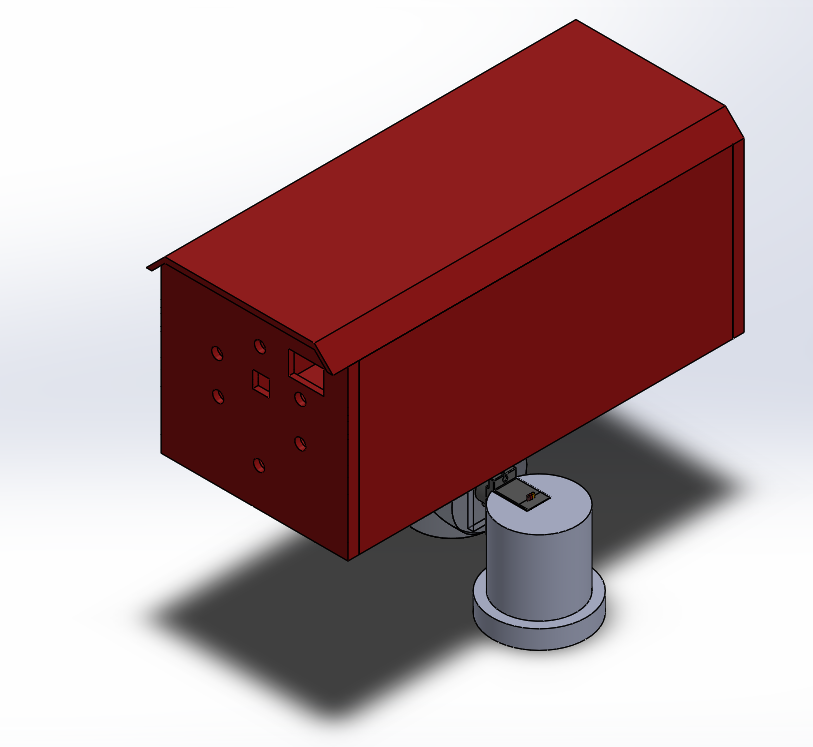
\includegraphics{media/Mark__00.png}
    \end{adjustbox}
    \caption{\label{fig:isometrico_Mark00}Vista Isometrica de la version Mark 0.}
    \end{figure}
    El prototipo representado en la Figura \ref{fig:isometrico_Mark00} corresponde a la primera iteración del diseño. En esta versión inicial, se puede apreciar que la concepción original se basaba en una estructura de forma rectangular, con la placa de potencia y control ubicada en la parte frontal, incluyendo orificios específicos para alojar la ESP32-CAM y los LEDs infrarrojos. Se había contemplado la posibilidad de ubicar un ventilador en la parte trasera para proporcionar la refrigeración del sistema en su totalidad.
    \begin{figure}[H]
    \centering
    \begin{adjustbox}{width=\linewidth/2}
      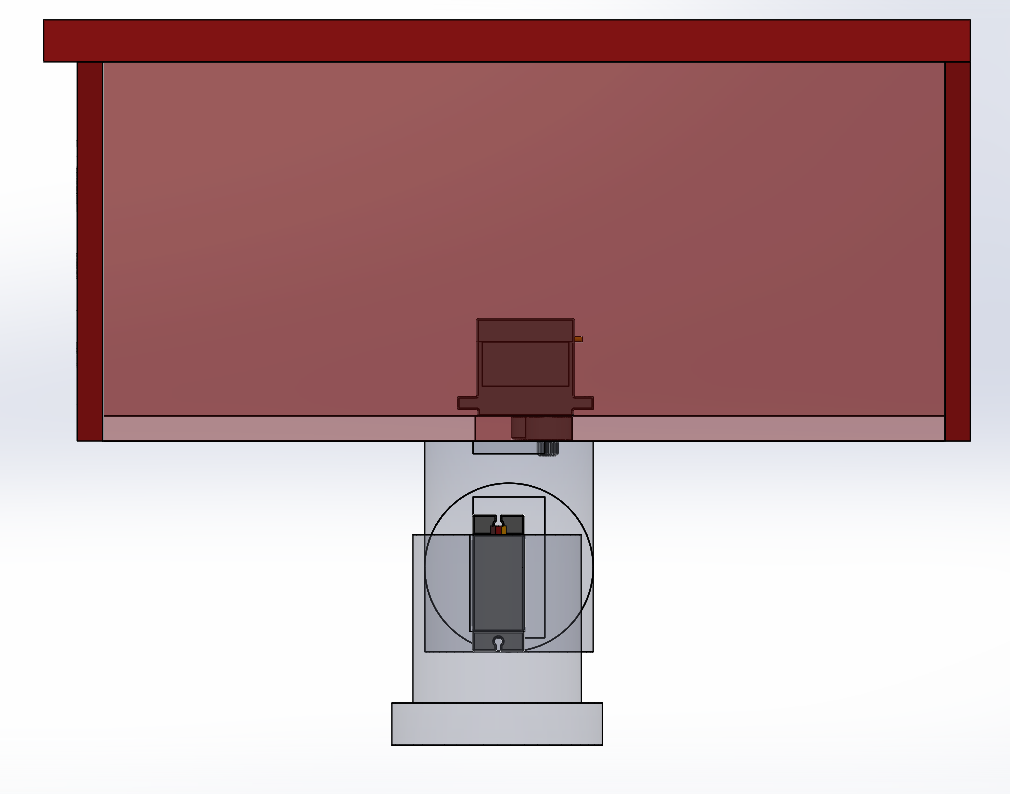
\includegraphics{media/lateral_Mark00.png}
    \end{adjustbox}
    \caption{\label{fig:lateral_Mark00}Vista Lateral de la version Mark 0.}
    \end{figure}
    En la Figura \ref{fig:lateral_Mark00}, se aprecia la posición estratégica de los servomotores empleados, los cuales desempeñan un papel fundamental al posibilitar el movimiento de la cámara en los ejes X e Y. En un principio, se había contemplado la posibilidad de albergar todos los sensores y demás dispositivos electrónicos dentro de la caja; no obstante, al encontrarse en una fase de concepción temprana, esta idea no llegó a concretarse.

\needspace{3cm}
\subsection{Mark I}
    \begin{figure}[H]
    \centering
    \begin{adjustbox}{width=\linewidth/2}
      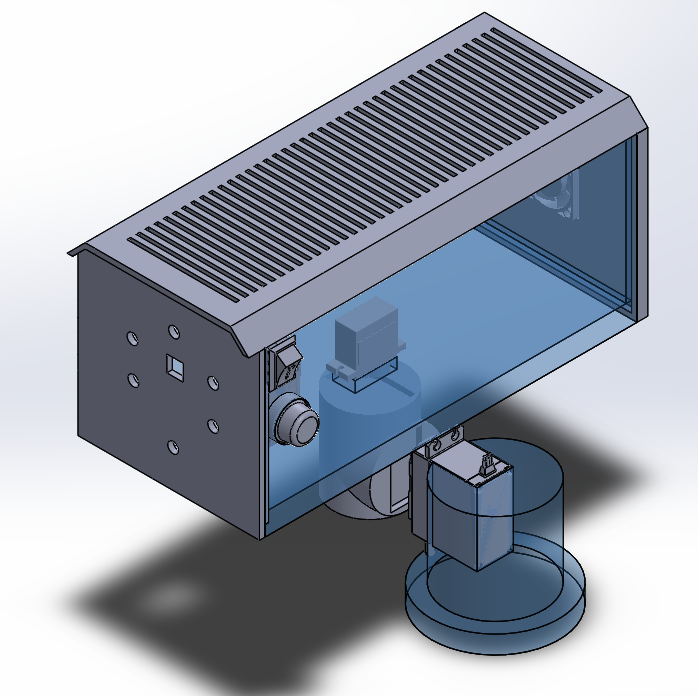
\includegraphics{media/Mark__01.png}
    \end{adjustbox}
    \caption{\label{fig:isometrico_Mark01}Vista Isometrica de la version Mark I.}
    \end{figure}
     El modelo exhibido en la Figura \ref{fig:isometrico_Mark01} representa la segunda etapa de desarrollo de este diseño. En esta iteración, se observa un notable progreso al incorporar diversos componentes clave, como el ventilador, el sensor de humo y un interruptor para alimentar todo el sistema. Además, se han añadido rejillas en la parte superior de la cámara para potenciar la refrigeración del sistema. Cabe destacar que los servomotores se mantuvieron en su posición original, con sus mismos soportes, conservando su funcionalidad anterior.
     Ademas, se mantuvo la idea de colocar la placa de potencia y control en la parte delantera de la camara, con los agujeros respectivos para alojar la ESP32-CAM y los LEDs infrarrojos.

\needspace{3cm}
\subsection{Mark II}
    \begin{figure}[H]
    \centering
    \begin{adjustbox}{width=\linewidth/2}
      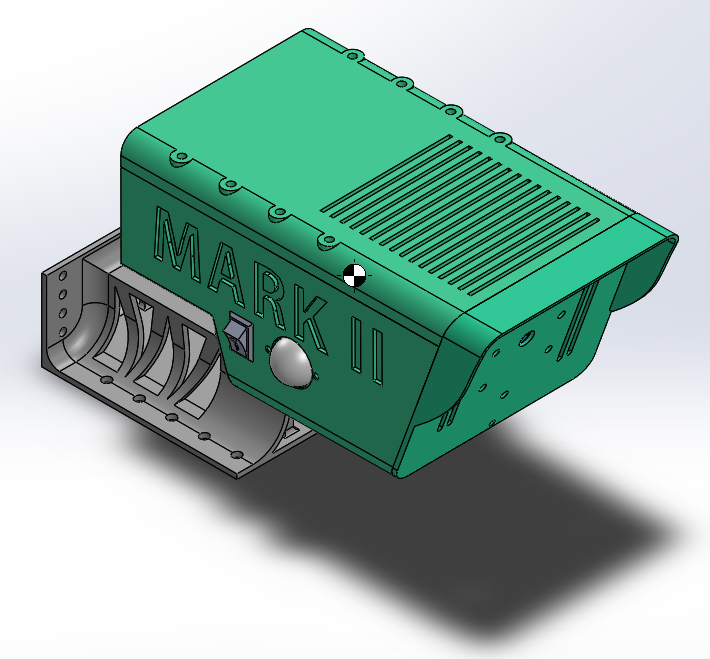
\includegraphics{media/Mark__02.png}
    \end{adjustbox}
    \caption{\label{fig:isometrico_Mark02}Vista Isometrica de la version Mark II.}
    \end{figure}

    En la Figura \ref{fig:isometrico_Mark02}, se pone de manifiesto la tercera fase de evolución en el diseño. En esta iteración, destacan cambios significativos, como la reubicación de la rejilla destinada a mejorar la refrigeración, la implementación de un soporte integral para la cámara, y la configuración que permite retirar la tapa superior para acceder y manipular los componentes electrónicos internos. Además, se han añadido rejillas de menor tamaño en la tapa superior, debido al incremento en la cantidad de componentes electrónicos empleados.

    \begin{figure}[H]
    \centering
    \begin{adjustbox}{width=\linewidth/2}
      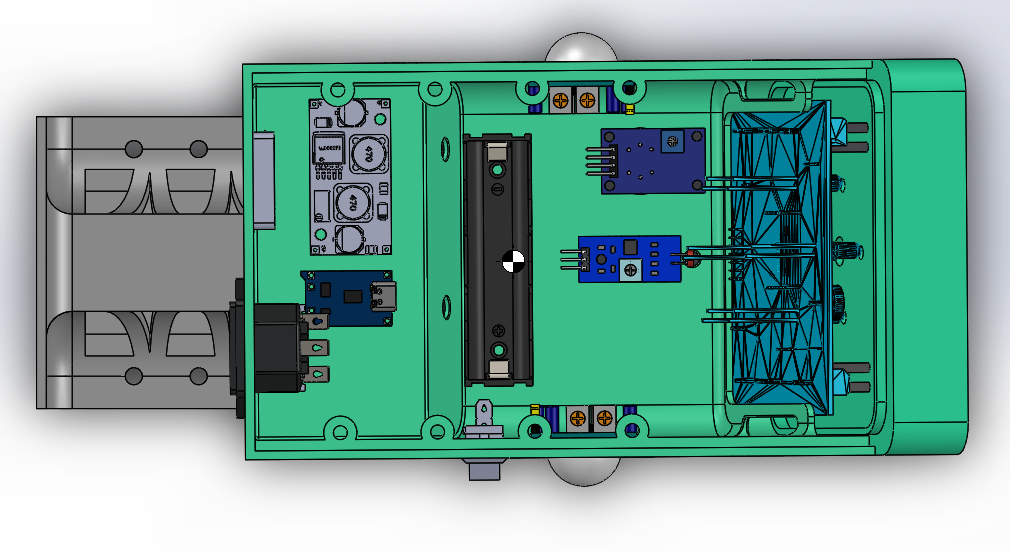
\includegraphics{media/superior_Mark02.png}
    \end{adjustbox}
    \caption{\label{fig:superior_Mark02}Vista Superior de la version Mark II.}
    \end{figure}    

    En la Figura \ref{fig:superior_Mark02}, se aprecia con claridad que el modelo Mark II se estaba destacando como el vencedor, lo que impulsó la incorporación de la totalidad de los componentes electrónicos previstos. El diseño original contemplaba la posibilidad de alimentar el sistema tanto con Corriente Alterna como con una batería en caso de cortes eléctricos. Para hacerlo factible, se implementó el módulo TP4056, que permitía cargar y activar dicha batería. Asimismo, se instaló un elevador de voltaje XL6009. Todos los sensores empleados desempeñaron roles específicos en la funcionalidad del dispositivo: dos sensores PIR en los laterales para activarse ante la detección de movimiento, un sensor de humo en la parte inferior para capturar imágenes en caso de detectar humo, y un LDR para activar los LEDs infrarrojos en condiciones de baja iluminación.

    \begin{figure}[H]
    \centering
    \begin{adjustbox}{width=\linewidth/2}
      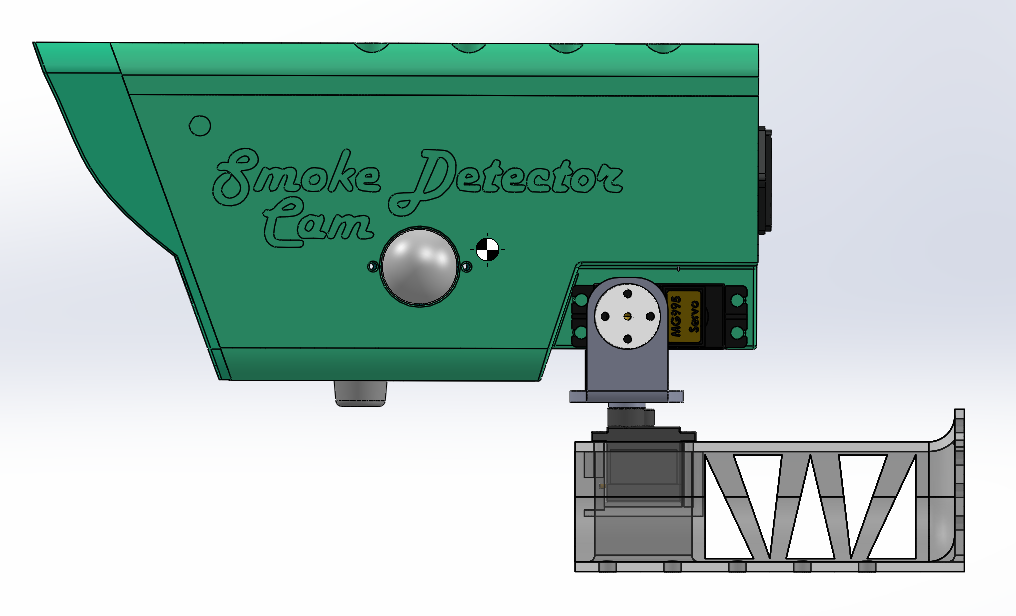
\includegraphics{media/posterior_Mark02.png}
    \end{adjustbox}
    \caption{\label{fig:posterior_Mark02}Vista Posterior de la versión Mark II.}
    \end{figure}

    En la Figura \ref{fig:posterior_Mark02} se aprecia que la ubicación de los servomotores se mantienen pero el soporte de los mismos se cambio. El primer cambio fue el soporte para instalar la cámara a la pared, de forma que se podría colocar y soportar el peso de la cámara. Además, de una pieza para que la cámara pueda rotar con facilidad sobre el eje Y.

    Cabe mencionar que en todas estas iteraciones se mantuvo la ubicación del ventilador para la refrigeración de los componentes electrónicos.

%\needspace{3cm}
\subsection{Mark III}
    En el Mark III se desarrolló un cambio total del sistema, forma y mecanismo de funcionamiento de la cámara tras aplicar e método de diseño y análisis de los cinco pasos.
    Se puede apreciar en la Figura~\ref{fig:Mark03} que el modelo obtenido es mucho mas parecido a una cámara moderna que en las versiones anteriores.
    
    \begin{figure}[H]
    \centering
    \begin{adjustbox}{width=\linewidth}
      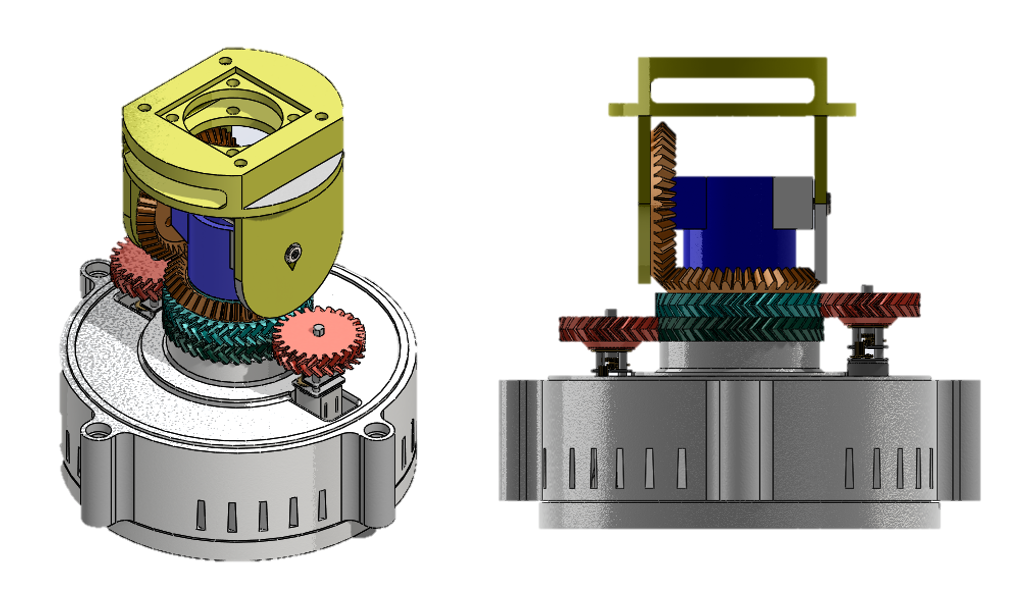
\includegraphics{media/mecanismo_Mark03.png}
    \end{adjustbox}
    \caption{\label{fig:mecanismo_Mark03} Mecanismo de la versión Mark III.}
    \end{figure}

    En la Figura \ref{fig:mecanismo_Mark03} se puede apreciar el mecanismo que queda claro en el cuadro \ref{tab:combinacion_3}, que es el Tren de Engranes Diferencial, usando motores DC y cada uno con una velocidad angular de 100rpm, de esta forma se tiene un movimiento de 600°/seg.
    La relacion de los engranes es que lo de los laterales (color rojo) tienen 24 dientes y los dos engranes grandes (los equivalente a color verde) tienen 40 dientes.

    \begin{figure}[H]
    \centering
    \begin{adjustbox}{width=\linewidth/3}
      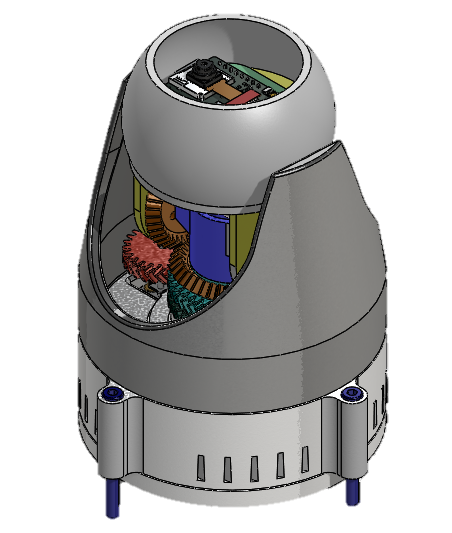
\includegraphics{media/vista_isometrica.png}
    \end{adjustbox}
    \caption{\label{fig:Mark03} Vista Isometrica de la versión Mark III.}
    \end{figure}

    En la Figura \ref{fig:Mark03}, se presenta una visión detallada del mecanismo de la cámara dentro de su elegante carcasa. Se destaca especialmente el movimiento preciso que ejecuta este mecanismo para posicionar la cámara en el ángulo exacto necesario para capturar la imagen de la persona que está fumando. Es importante señalar que todo el sistema de alimentación y placa de potencia se ubican en la parte inferior de la estructura. En la parte superior, justo debajo de la ESP32-CAM, se encuentra el ventilador, mientras que las rejillas en la parte inferior permiten la refrigeración de la placa de potencia. El flujo del aire de refrigeración para este prototipo se puede apreciar en la Figura~\ref{fig:flujoDeAire}. Seria este mismo canal común dentro del cual se tienen que ordenar los cables y conexiones de los dispositivos electrónicos del sistema.

    \begin{figure}[H]
    \centering
    \begin{adjustbox}{width=\linewidth}
    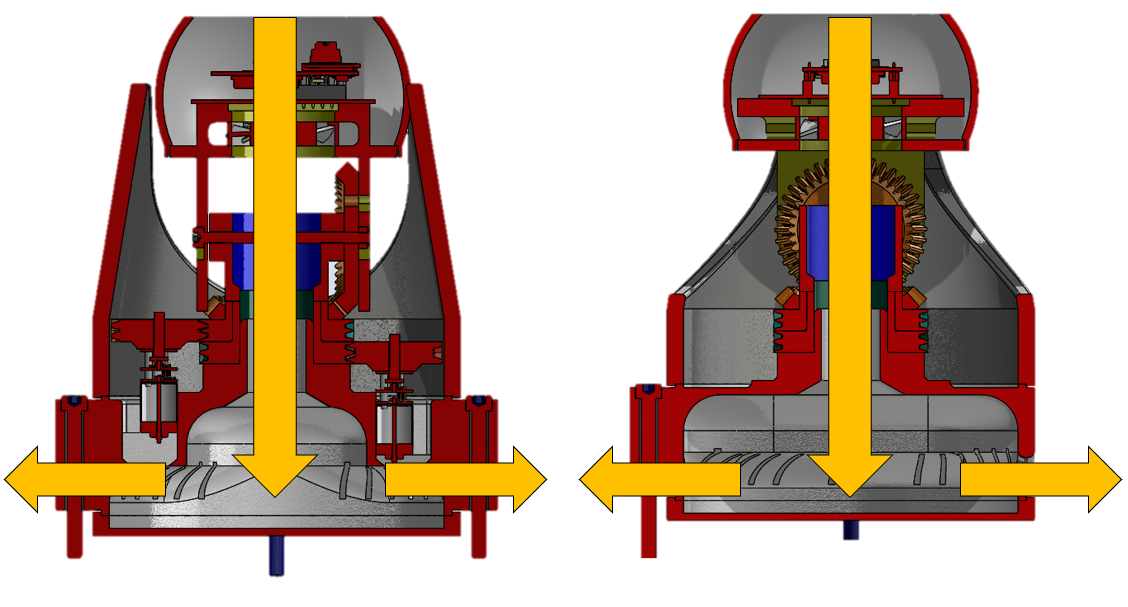
\includegraphics{media/vista_seccion_aire.png}
    \end{adjustbox}
    \caption{\label{fig:flujoDeAire} Vista de sección de la cámara en la que se puede apreciar el flujo de aire empujado por el ventilador planteado mediante las fechas amarillas.}
    \end{figure}

    \subsubsection{Base de la Cámara}
    La base de la cámara se diseñó con un enfoque primordial en el mecanismo que debía ubicarse sobre ella, así como en los componentes que debían ser alojados en su interior. Estos componentes incluían la unidad de potencia, módulos de posible expansión, conductos de refrigeración, baterías, el método de sujeción, la facilidad de impresión 3D y, por último, la estética del producto.

    A partir del complejo mecanismo de transmisión de movimiento, compuesto por una variedad de engranajes, se logró desarrollar la forma del encapsulado de manera orgánica. Se creó una base circular hueca diseñada para albergar los componentes de potencia en su interior, con orificios estratégicos destinados a sujetar los motores DC mediante un apriete preciso. Además se trató de mantener las secciones sobresalientes a mas de 45 grados tal y como propone \cite{Redwood_2017} a fin de no necesitar soportes para la impresión de la misma o en su defecto de mantener los puentes con un longitud igual o inferior a un centímetro.
    
    En cuanto a la sujeción, se planteó la utilización de tres tornillos, y la posición del cuarto tornillo fue sustituida por un agujero que permitía el paso de los cables de alimentación, manteniendo así la integridad de la estética del producto.
    
    \subsubsection{Engranes Helicoidales}
    Los engranes helicoidales destacan como una elección sobresaliente en la concepción de mecanismos para sistemas de impresión 3D ya que su mayor complejidad geométrica no implica un mayor costo de producción o necesidad de remover soportes. Su característica más distintiva radica en la inclinación helicoidal de los dientes en lugar de ser perpendiculares al eje de rotación. Esta inclinación suave desempeña un papel fundamental en la reducción de ruido y vibraciones.
    Además de la reducción de ruido y las ventajas en la capacidad de carga, es esencial entender cómo se llevó a cabo la reducción de velocidad mediante el uso de engranes en tu sistema. En tu caso, tienes un motor con una velocidad de entrada de 100 RPM, y en su eje hay un engrane con 24 dientes conectado a otro con 40 dientes. Para calcular la reducción de velocidad que este conjunto de engranes proporciona se utiliza la siguiente fórmula:

    \begin{equation}
    \text{Reducción de velocidad} = \frac{\text{Número de dientes del engrane conductor}}{\text{Número de dientes del engrane conducido}}
    \end{equation}
    
    En este caso, el engrane conductor es el que tiene 24 dientes, y el engrane conducido es el de 40 dientes, por lo que la reducción de velocidad es:
    
    \begin{equation*}
    \text{Reducción de velocidad} = \frac{24}{40} = 0.6
    \end{equation*}
    
    Esto significa que el sistema de engranes reduce la velocidad del motor en un 60\%.
    La elección del módulo y el número de dientes en los engranes fue un proceso iterativo que involucró la optimización tanto de la estética como del tamaño del sistema, al mismo tiempo que se buscaba reducir la velocidad de los motores.
    
    \subsubsection{Engranes Cónicos}
    Los engranes cónicos permiten la transferencia de movimiento rotacional de un plano a otro con un ángulo de desviación, esencial para mantener una transmisión de potencia eficiente en el mecanismo diferencial. En este caso se colocaron a 45 grados para poder mover la cámara en los ejes planteados, mismos que son normales el uno del otro.

    \subsubsection{Torreta}
    La torreta se posiciona como una pieza central del mecanismo, permite posicionar el eje del brazo, así como sincronizar el movimiento de uno de los engranes helicoidales con el movimiento sobre el plano de planta que debe realizar la cámara. Adicionalmente, al ser hueco funciona como conducto de aire de refrigeración.
    
    \subsubsection{Brazo}
    El brazo del mecanismo permite conectar el efector final al mecanismo por medio de pernos y ejes que lo alinean al mismo. En el Mark III se colocaron la placa de control en donde se sitúa la cámara así como el ventilador al final del brazo. Más aun, se tomó en cuenta la posición de impresión del brazo al momento de diseñar las sujeciones laterales. Estos agujeros presentan formas de gota de agua, esto debido a que se agrega un ángulo por la parte superior de los orificios para evitar el uso de soportes al momento de impresión. En este caso la gota tiene un ángulo de sesenta grados lo que permite impresión sin problemas en materiales como el ABS o el PLA sin problemas. El ángulo se puede disminuir hasta cuarenta  cinco grados en caso de limitarse utilizar PLA.
    Se diseñaron dos modelos: Uno con frente recto y otro con frente redondeado.
    
    \subsubsection{Carcasa}
    Finalmente la carcasa exterior tiene la función de resguardar el mecanismo en su interior sin perjudicar el movimiento del mecanismo. Tratando de imitar las cámaras modernas, tales como la descrita en la Figura~\ref{fig:Imou} se diseñó uno compuesto por una carcasa exterior con conjunto con un esferoide posicionado mediante apriete alrededor de la cámara conectada en el brazo. 

    \needspace{6cm}
    \subsection{Mark IV}

    \begin{figure}[H]
    \centering
    \begin{adjustbox}{width=0.7\linewidth}
      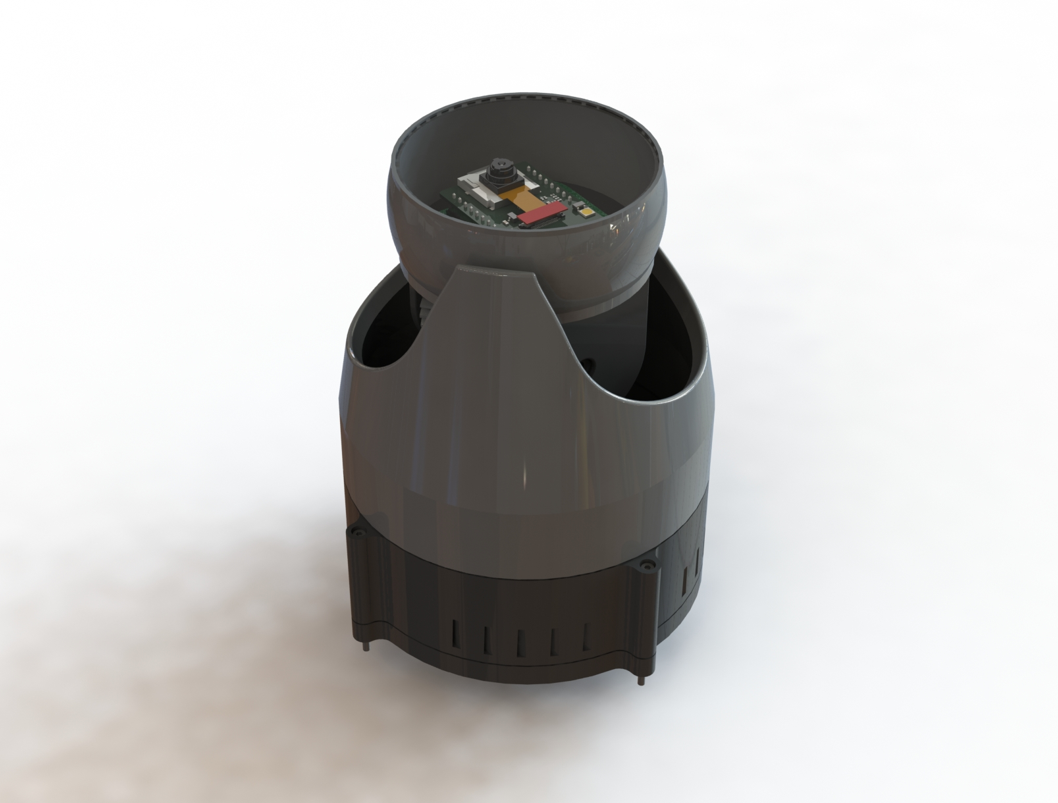
\includegraphics{media/markiv/vista_isometricaf.png}
    \end{adjustbox}
    \caption{\label{fig:Mark04} Vista Isometrica Renderizada de la versión Mark IV.}
    \end{figure}

    En la versión Mark IV se modificó la posición del ventilador en el ensamble. Pasando de estar montado en el brazo junto a la sección de control a estar montado en la torreta por encima de la sección de potencia. Respetando de igual manera el flujo de aire explicado en la Figura~\ref{fig:flujoDeAire}.
    
    \subsubsection{Torreta}

    \begin{figure}[H]
    \centering
    \begin{adjustbox}{width=0.7\linewidth}
      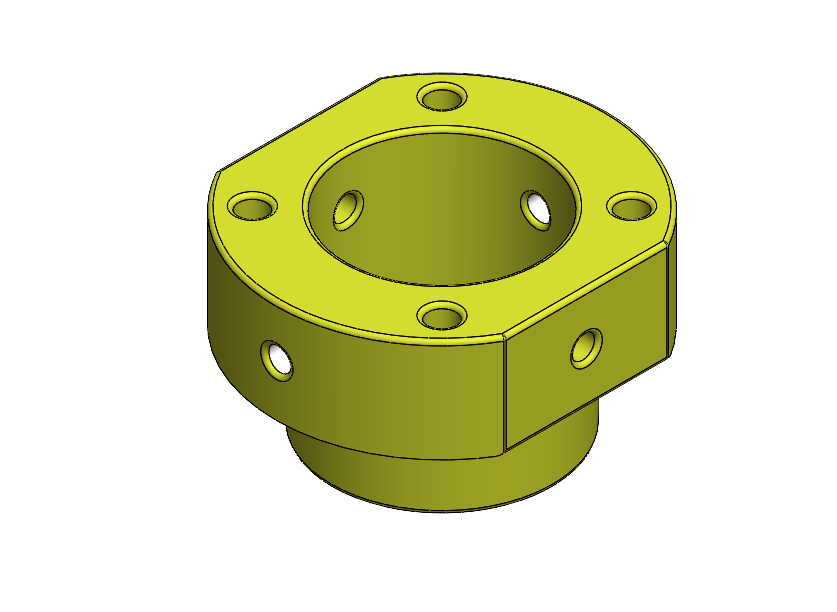
\includegraphics{media/markiv/torreta.png}
    \end{adjustbox}
    \caption{\label{fig:torretaMarkIV} Vista Isometrica de la Torreta modificada en la versión Mark IV.}
    \end{figure}
    
    La Figura~\ref{fig:torretaMarkIV} muestra los cambios realizados en la Torreta para permitir el montaje del ventilador por encima de la misma de manera que la sección de potencia cuente siempre con un flujo constante de aire en su interior.
    
    \subsubsection{Brazo}

    \begin{figure}[H]
    \centering
    \begin{adjustbox}{width=0.7\linewidth}
      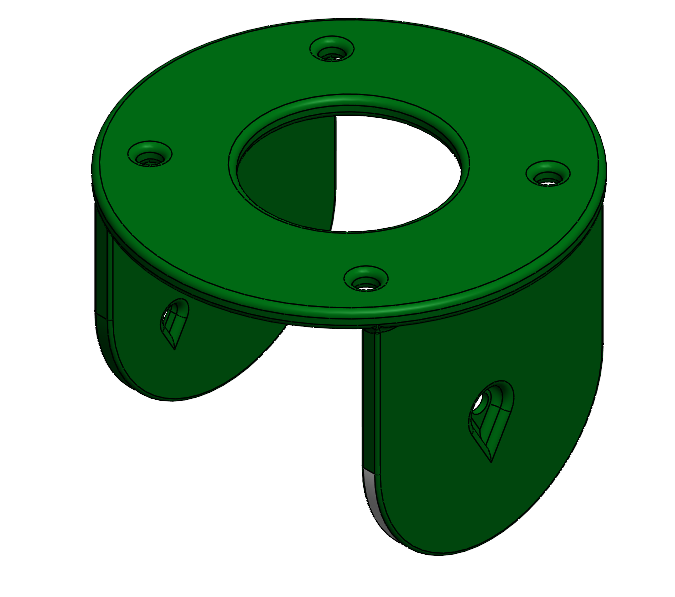
\includegraphics{media/markiv/brazo.png}
    \end{adjustbox}
    \caption{\label{fig:brazoMarkIV} Vista Isometrica del Brazo modificado en la versión Mark IV.}
    \end{figure}

     La Figura~\ref{fig:brazoMarkIV} permite apreciar que al no tener una abertura para colocar el ventilador el diseño del brazo que sostiene al circuito de control se ve simplificado, permitiendo su impresión en maquinas FDM sin soportes.